\chapter{Lecture 7 - Introduction to Linear Algebra and Gauss Elimination}
\label{ch:lec7n}
\section{Objectives}
The objectives of this lecture are to:
\begin{itemize}
\item Provide background and describe why engineers what to solve systems of linear equations.
\item Describe and demonstrate the Gauss elimination algorithm.
\item Do an example in MATLAB.
\end{itemize}
\setcounter{lstannotation}{0}

\section{Background}

Linear systems of equations arise in a variety of contexts.  For example, consider a simple analysis of a truss structure as shown in Figure \ref{fig:lec7n-truss}.  If you are to conduct a simple static analysis of this structure, you would need to derive equilibrium equations to show that the sum of forces at each point---A, B, C, D, E, and F---in the $x$- and $y$-direction equals zero.  A total of eight equations are drived in this way and shown below.
\begin{marginfigure}
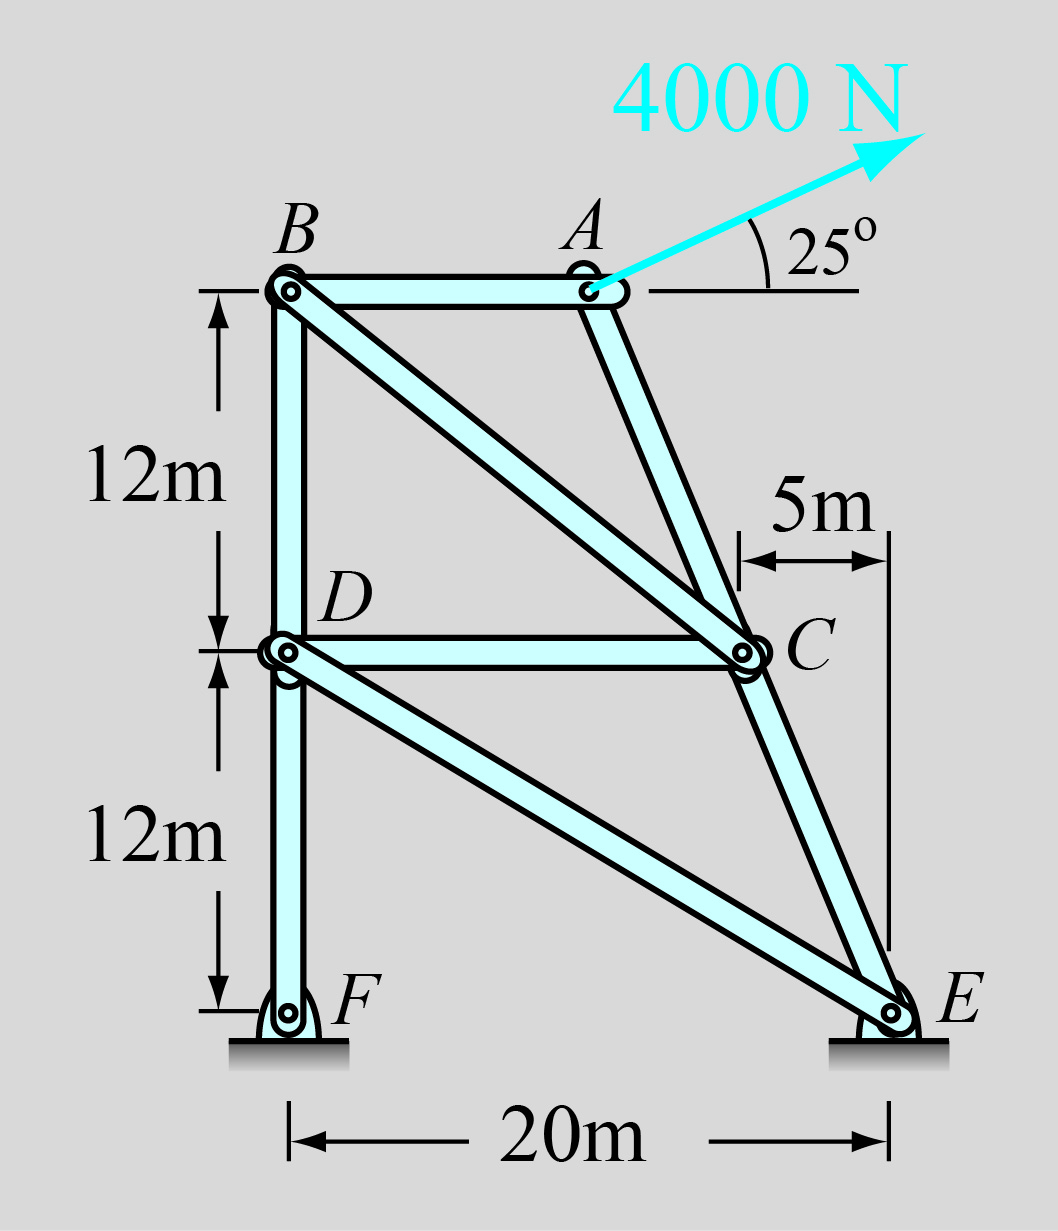
\includegraphics{Chapter4Example4_3.jpg}
\caption{Two-dimensional truss structure.}
\label{fig:lec7n-truss}
\end{marginfigure}
%\begin{fullwidth}
\begin{centering}
\begin{table}
\begin{tabular}{l l l}
$-F_{AB} - 0.3846F_{AC} = 3625$ & $0.9231F_{AC} = 1690$ & $\sum F_{x}$, $\sum {F_y}$ at A \\
$F_{AB} - 0.7809 F_{BC}=0$ & $0.6247F_{BC} - F_{BD} = 0$ & $\sum F_{x}$, $\sum {F_y}$ at B\\
\multicolumn{2}{l}{$- 0.3846F_{AC} - 0.7809F_{BC} - F_{CD} + 0.3846F_{CE}  = 0$} & $\sum F_{x}$ at C \\
\multicolumn{2}{l}{$0.9231F_{AC}+0.6247F_{BC} - 0.9231F_{CE} = 0$} & $\sum F_{y}$ at C \\
$F_{CD}+0.8575F_{DE} = 0$ & $F_{BD} - 0.5145F_{DE} - F_{DF} = 0$ & $\sum F_{x}$, $\sum {F_y}$ at D\\
\end{tabular}
\end{table}
\end{centering}
%\end{fullwidth}
We cannot, in general, solve these equations individually, the unknown values---the tension in each of the eight truss elements---are distributed among all of the equations.  In general we must solve the equations simultaneously; the resulting linear equations are shown in matrix-vector form in Equation \ref{eq:lec7n-truss-soe}.
\begin{fullwidth}
\begin{equation}
\left[
\begin{matrix}
-1 & -0.3846 & 0 & 0 & 0 & 0 & 0 & 0 \\
0 & 0.9231 & 0 & 0 & 0 & 0 & 0 & 0 \\
1 & 0 & -0.7809 & 0 & 0 & 0 & 0 & 0 \\
0 & 0 & 0.6247 & -1 & 0 & 0 & 0 & 0 \\
0 & -0.3846 & -0.7809 & 0 & -1 & 0.3846 & 0 & 0 \\
0 & 0.9231 & 0.6247 & 0 & 0 & -0.9231 & 0 & 0 \\ 
0 & 0 & 0 & 0 & 1 & 0 & 0.8575 & 0 \\
0 & 0 & 0 & 1 & 0 & 0 & -0.5145 & - 1 \\
\end{matrix}
\right]
\left[
\begin{matrix}
F_{AB} \\
F_{AC} \\
F_{BC} \\
F_{BD} \\
F_{CD} \\
F_{CE} \\
F_{DE} \\
F_{DF} 
\end{matrix}
\right]
=
\left[
\begin{matrix}
3625 \\
1690 \\
0 \\
0 \\
0 \\
0 \\
0 \\
0 \\
\end{matrix}
\right]
\label{eq:lec7n-truss-soe}
\end{equation}
\end{fullwidth}

A second, and perhaps more generally relevant case, is when a linear differential operator is represented in a discrete form.  Consider the boundary value problem expressed in Equation \ref{eq:lec7n-bvp-ex}.
\begin{equation}
\frac{d^2 u}{d x^2} = f(x), \ \ 0 < x < L, \ \ u(0) = u(L) = 0
\label{eq:lec7n-bvp-ex}
\end{equation}
As we will study later in this course, the spatial domain $x \in [0,L]$ can be discretized into uniform segements, the differential operator $\sfrac{d^2}{dx^2}$, the solution $u(x)$, and the input function $f(x)$ can all be expressed in a discrete form and assembled into a system of linear equations.  This is shown in Equation \ref{eq:lec7n-bvp-ex-discrete}:
\marginnote{In this expression we use the second-order central difference approximation to $\sfrac{d^2u}{dx^2}$ which is:
$$ \frac{d^2u}{dx^2} = \frac{u(x_{i-1}) - 2u(x_i) + u(x_{i+1})}{h^2}$$
and a matrix is formed from the resulting system of equations.  The first and last row of the matrix along with the first and last element of $f(x_i)$ are modified to satisfy the given boundary conditions. These techniques will be discussed more fully when we present finite difference methods for solving boundary value problems.
}
\begin{equation}
\underbrace{
\frac{1}{h^2}
\left[
\begin{matrix}
1 & 0 & 0 & \cdots & \cdots &  0 \\
1 & -2 & 1 & 0 & \cdots & \vdots \\
0 & \ddots & \ddots & \ddots & \ddots& \vdots \\
\vdots &  \ddots & 1 & -2 & 1 &  0 \\
\vdots & \cdots & \ddots & 1 & -2 & 1  \\
0 & \cdots & \cdots & 0 & 0 & 1
\end{matrix}
\right]
}_{\frac{d^2}{dx^2}, \ \  u(0)=u(L)=0}
\underbrace{
\left[
\begin{matrix}
u(x_0) \\
u(x_1) \\
\vdots \\
\vdots \\
u(x_{n-1}) \\
u(x_n)
\end{matrix}
\right]
}_{u(x)}
=
\underbrace{
\left[
\begin{matrix}
0 \\
f(x_1) \\
\vdots \\
\vdots \\
f(x_{n-1}) \\
0
\end{matrix}
\right]
}_{\substack{f(x) \\ \text{with BC}}}
\label{eq:lec7n-bvp-ex-discrete}
\end{equation}
where $h = x_{i+1} - x_i$.  Depending on how accurate of a solution is desired, the system illustrated in Equation \ref{eq:lec7n-bvp-ex-discrete} can have thousands of equations or more.  For a known $f(x)$, we can use the methods we will describe in this and the next few lectures to solve the equations to find $u(x)$.

\section{Gauss Elimination}
Gauss elimination is the most basic \emph{direct} method\sidenote{In later lectures we will describe \emph{iterative} methods for solving linear systems of equaions.  In iterative methods we start with an initial guess of the solution vector and iteratively improve upon it.  Eventually a solution is obtained but the number of operations required cannot be determined in advance.} for solving systems of linear equations.  When it succeeds, the system of equations is solved within a pre-determined number of mathematical operations.

\newthought{The basic procedure} is done in two steps.  First we start with a system of equations that includes a square, invertible matrix:
\begin{equation*}
\bracketMatrixstack{
a_{11} &  a_{12} & \cdots & a_{1n} \\
a_{21} & a_{22} & \cdots & a_{2n} \\
\cdots & \ddots & \ddots & \vdots \\
a_{n1} & a_{n2} & \cdots & a_{nn} 
}
\bracketVectorstack{
x_1 \\
x_2 \\
\vdots \\
x_n
} =
\bracketVectorstack{
b_1 \\
b_2 \\
\vdots \\
b_n
}
\end{equation*} 
and convert it to an upper-tringular matrix using a matrix called \emph{forward elimination}.
\begin{equation*}
\bracketMatrixstack{
a_{11} & a_{12} & \cdots & a_{1n} \\
0 & a^{\prime}_{22} & \cdots & a^{\prime}_{2n} \\
\vdots & \ddots & \ddots & \vdots \\
0 & \cdots & 0 & a^{\prime}_{nn}
} 
\bracketVectorstack{
x_1 \\
x_2 \\
\vdots \\
x_n
}
=
\bracketVectorstack{
b^{\prime}_1 \\
b^{\prime}_2 \\
\vdots \\
b^{\prime}_n
}
\end{equation*}
The resulting upper-triangular matrix can readily be solved in a process called \emph{back substitution}.
